\documentclass{article}

\usepackage{graphicx}
\usepackage[left=2.5cm, right=2.5cm, top=2cm, bottom=2cm]{geometry}
\usepackage{titlesec}
\usepackage{amsmath}
\usepackage{algorithm}
\usepackage{algpseudocode}
\usepackage{tikz}
\usepackage{caption}
\usepackage{listings}
\usepackage{xcolor}
\usepackage{fancyhdr}
\usepackage{changepage}
\usepackage{svg}
\usepackage{float} % 提供更灵活的图片位置控制
\usepackage{booktabs}
\usepackage{minted}
\pagestyle{fancy}
\fancyhf{} % 清空页眉和页脚
\fancyfoot[C]{\thepage} % 只在页脚中居中显示页码
\renewcommand{\headrulewidth}{0pt} % 去掉页眉的横线
\usetikzlibrary{trees, shapes.geometric, arrows, positioning}
\usepackage{lmodern}
\usepackage[UTF8]{ctex}
\usepackage{xeCJK}
    \setCJKmainfont[AutoFakeBold=3]{TW-Sung}
    \XeTeXlinebreaklocale "zh"
    \XeTeXlinebreakskip = 0pt plus 1pt
\usepackage{multirow}
\ctexset{
    figurename = {Figure},
    tablename = {Table}
}
\definecolor{bg}{rgb}{0.95,0.95,0.92} % 定義一個自定義顏色
\definecolor{lightgray}{gray}{0.9} % 設定一個淺灰色

\titleformat{\section}[hang]{\normalfont\Large\bfseries}{\thesection}{1em}{}
\titleformat{\subsection}[hang]{\normalfont\bfseries}{\thesubsection}{2em}{}
\titleformat{\subsubsection}[hang]{\normalfont\bfseries}{\thesubsubsection}{5em}{}

\titlespacing*{\subsection}{2em}{3.25ex plus 1ex minus .2ex}{1.5ex plus .2ex}
\titlespacing*{\subsubsection}{3em}{3.25ex plus 1ex minus .2ex}{1.5ex plus .2ex}

% 定義 SQL 的語法高亮
\lstdefinelanguage{SQL}{
    keywords={SELECT, FROM, WHERE, INSERT, UPDATE, DELETE},
    keywordstyle=\color{blue},
    commentstyle=\color{brown},
    stringstyle=\color{red}
}

% 定義 Python 的語法高亮
\lstdefinelanguage{Python}{
    keywords={def, return, if, else, import, print},
    keywordstyle=\color{green},
    commentstyle=\color{gray},
    stringstyle=\color{orange}
}

% 全局設置
\lstset{
    basicstyle=\ttfamily\small,
    showstringspaces=false,
    numbers=left,
    numberstyle=\tiny\color{gray},
    stepnumber=1,
    numbersep=5pt,
    backgroundcolor=\color{white},
    frame=single,
    rulecolor=\color{black},
    captionpos=b,
    inputencoding=utf8,
    extendedchars=true
}



\title{Database Management\\Homework 3}
\author{B11705044 \\ Yen-Hung, Chiang}
\date{}

\begin{document}

\maketitle

\section*{1}
\subsection*{(a)}
根據題目的敘述查詢到的員工編號有四個,下面為查詢的 SQL 程式碼。查詢結果如 Table \ref{table:1_a} 所表示。
\begin{minted}[bgcolor=lightgray, linenos]{SQL}
SELECT 
    E.Ssn, 
    E.Bdate, 
    COUNT(DISTINCT DEP.Dependent_name) AS dependent_count
FROM 
    EMPLOYEE E
JOIN 
    DEPARTMENT D ON E.Dno = D.Dnumber 
JOIN 
    DEPT_LOCATIONS DL ON D.Dnumber = DL.Dnumber 
LEFT JOIN 
    DEPENDENT DEP ON E.Ssn = DEP.Essn 
GROUP BY 
    E.Ssn, E.Bdate
HAVING 
    COUNT(DISTINCT DL.Dlocation) > 1
ORDER BY
    E.Ssn;
\end{minted}
\begin{table}[H]
\centering
\begin{tabular}{ccc}
\toprule
Ssn & Bdate & dependent\_count \\
\midrule
123456789 & 1965-01-09 & 3 \\
333445555 & 1955-12-08 & 3 \\
453453453 & 1972-07-31 & 0 \\
666884444 & 1962-09-15 & 0 \\
\bottomrule
\end{tabular}
\caption{Employee Information with Birthdate and Dependent Count}
\label{table:1_a}
\end{table}



\subsection*{(b)}
根據題目的敘述有兩個部門符合條件,下面為查詢所需的 SQL 程式碼。查詢的結果如 Tablel \ref{table:1_b} 所表示
\begin{minted}[bgcolor=lightgray, linenos, breaklines=true]{SQL}
SELECT
    D.Dnumber AS Department_Number,  
    D.Dname AS Department_Name,
    FLOOR(AVG(FLOOR(DATE_PART('year', AGE('2024-10-01', E.Bdate))))) AS Average_Age
FROM
    EMPLOYEE E
JOIN
    DEPARTMENT D ON E.Dno = D.Dnumber
GROUP BY
    D.Dnumber, D.Dname
HAVING 
    COUNT(E.Ssn) > 1;
\end{minted}
\begin{table}[H]
\centering
\begin{tabular}{ccc}
\toprule
DNumber & DName & Average\_Age \\
\midrule
4 & Administration & 64 \\
5 & Research & 60 \\
\bottomrule
\end{tabular}
\caption{Average Age of Employees in Departments with More Than Two Employees}
\label{table:1_b}
\end{table}

\subsection*{(c)}
根據題目的敘述要查詢的條件為參與人數第二多的專案,由於 (e) 小題裡面有提到如果有某個人在某個專案的工時為 NULL 就忽略那筆資料,最後查詢出來的結果有三個專案並列第二名,下面是查詢所需的 SQL 程式碼。查詢結果如 Table \ref{table:1_c} 所表示。
\begin{minted}[bgcolor=lightgray, linenos]{SQL}
WITH ProjectParticipation AS (
    SELECT 
        P.Pnumber AS Project_Number,
        P.Pname AS Project_Name,
        COUNT(W.Essn) AS Participant_Count,  
        AVG(W.Hours) AS Average_Hours         
    FROM 
        PROJECT P
    LEFT JOIN 
        WORKS_ON W ON P.Pnumber = W.Pno
    WHERE 
        W.Hours IS NOT NULL  
    GROUP BY 
        P.Pnumber, P.Pname
),
RankedProjects AS (
    SELECT 
        Project_Number,
        Project_Name,
        Average_Hours,
        Participant_Count,
        DENSE_RANK() OVER (ORDER BY Participant_Count DESC) AS Participation_Rank  
    FROM 
        ProjectParticipation
)

SELECT 
    Project_Number,
    Project_Name,
    Average_Hours
FROM 
    RankedProjects
WHERE 
    Participation_Rank = 2; 
\end{minted}
\begin{table}[H]
\centering
\begin{tabular}{ccc}
\toprule
Project\_Number & Project\_Name & Average\_Hours \\
\midrule
1 & ProductX & 26.25 \\
3 & ProductZ & 25.00 \\
20 & Reorganization & 12.50 \\
\bottomrule
\end{tabular}
\caption{Average Hours in Projects with Second Highest Participation}
\label{table:1_c}
\end{table}

\subsection*{(d)}
符合條件的員工總共有五位,下面為查詢所需的 SQL 程式碼。查詢結果如 Table \ref{table:1_d} 所表示。
\begin{minted}[bgcolor=lightgray, linenos]{SQL}
WITH ProjectParticipation AS (
    SELECT 
        P.Pnumber AS Project_Number,
        P.Pname AS Project_Name,
        COUNT(W.Essn) AS Participant_Count,  
        AVG(W.Hours) AS Average_Hours         
    FROM 
        PROJECT P
    LEFT JOIN 
        WORKS_ON W ON P.Pnumber = W.Pno
    WHERE 
        W.Hours IS NOT NULL  
    GROUP BY 
        P.Pnumber, P.Pname
),
RankedProjects AS (
    SELECT 
        Project_Number,
        Project_Name,
        Average_Hours,
        Participant_Count,
        DENSE_RANK() OVER (ORDER BY Participant_Count DESC) AS Participation_Rank  
    FROM 
        ProjectParticipation
)

SELECT 
    E.Ssn, 
    E.Lname, 
    CASE 
        WHEN E.Salary >= 40000 THEN 'yes' 
        ELSE 'no' 
    END AS Salary_Above_40k, 
    D.Mgr_ssn, 
    M.Lname AS Manager_Lname 
FROM 
    EMPLOYEE E
JOIN 
    WORKS_ON W ON E.Ssn = W.Essn
JOIN 
    PROJECT P ON W.Pno = P.Pnumber
JOIN 
    DEPARTMENT D ON E.Dno = D.Dnumber
JOIN 
    EMPLOYEE M ON D.Mgr_ssn = M.Ssn  
WHERE 
    P.Pnumber IN (
        SELECT Project_Number
        FROM RankedProjects
        WHERE Participation_Rank = 2  
    )
AND
    W.Hours IS NOT NULL
GROUP BY 
    E.Ssn, E.Lname, E.Salary, D.Mgr_ssn, M.Lname  
ORDER BY
    E.Ssn;
\end{minted}
\begin{table}[H]
\centering
\begin{tabular}{ccccc}
\toprule
Ssn & Lname & Salary\_Above\_40k & Mgr\_ssn & Manager\_Lname \\
\midrule
123456789 & Smith & no & 333445555 & Wong \\
333445555 & Wong & yes & 333445555 & Wong \\
453453453 & English & no & 333445555 & Wong \\
666884444 & Narayan & no & 333445555 & Wong \\
987654321 & Wallace & yes & 987654321 & Wallace \\
\bottomrule
\end{tabular}
\caption{Employees in Projects with Second Highest Participation}
\label{table:1_d}
\end{table}


\subsection*{(e)}
每位員工的參與的專案數、每週時數總和,以及其參與的專案跨幾個地點如 Table \ref{table:1_e} 所示,可以看到 \texttt{Ssn} 為 "888665555" 的這位員工並沒有參與任何專案,所以他的其餘欄位都是 0。下面是查詢所需的 SQL 程式碼。
\begin{minted}[bgcolor=lightgray, linenos]{SQL}
SELECT 
    E.Ssn,
    COALESCE(COUNT(DISTINCT W.Pno), 0) AS Project_Count,  
    COALESCE(SUM(W.Hours), 0) AS Total_Hours,              
    COALESCE(COUNT(DISTINCT P.Plocation), 0) AS Location_Count  
FROM 
    EMPLOYEE E
LEFT JOIN 
    WORKS_ON W ON E.Ssn = W.Essn AND W.Hours IS NOT NULL  
LEFT JOIN 
    PROJECT P ON W.Pno = P.Pnumber
GROUP BY 
    E.Ssn  
ORDER BY 
    E.Ssn;  
\end{minted}
\begin{table}[H]
\centering
\begin{tabular}{cccc}
\toprule
Ssn & Project\_Count & Total\_Hours & Location\_Count \\
\midrule
123456789 & 2 & 40.00 & 2 \\
333445555 & 4 & 40.00 & 3 \\
453453453 & 2 & 40.00 & 2 \\
666884444 & 1 & 40.00 & 1 \\
888665555 & 0 & 0 & 0 \\
987654321 & 2 & 35.00 & 2 \\
987987987 & 2 & 40.00 & 1 \\
999887777 & 2 & 40.00 & 1 \\
\bottomrule
\end{tabular}
\caption{Number of Project Participations for every Employee}
\label{table:1_e}
\end{table}


\subsection*{(f)}
所有沒有下屬的員工如 Table \ref{table:1_f} 所示,總共有五位員工沒有下屬。下面為查詢所需的 SQL 程式碼。
\begin{minted}[bgcolor=lightgray, linenos]{SQL}
SELECT 
    E.Ssn,
    COALESCE(COUNT(DISTINCT W.Pno), 0) AS Project_Count  
FROM 
    EMPLOYEE E
LEFT JOIN 
    EMPLOYEE S ON E.Ssn = S.Super_ssn
LEFT JOIN 
    WORKS_ON W ON E.Ssn = W.Essn
WHERE 
    S.Ssn IS NULL
GROUP BY 
    E.Ssn
ORDER BY 
    E.Ssn;
\end{minted}
\begin{table}[H]
\centering
\begin{tabular}{cc}
\toprule
Ssn & Project\_Count \\
\midrule
123456789 & 2 \\
453453453 & 2 \\
666884444 & 1 \\
987987987 & 2 \\
999887777 & 2 \\
\bottomrule
\end{tabular}
\caption{Project Count of Employees Without Subordinates}
\label{table:1_f}
\end{table}







\section*{2}
\subsection*{(a)}
根據題目的要求得到的查詢結果如 Table \ref{table:2_a} 所示。下面為這題的 Python 程式碼。
\begin{minted}[bgcolor=lightgray, linenos]{python}
import pandas as pd
import duckdb
import psycopg2

with open('password.txt', 'r') as file:
    password = file.read().strip()  

connection = psycopg2.connect(
    dbname='onlinelearning',
    user='postgres',  
    password=password,  
    host='localhost',
    port='5432'
)

answers_df = pd.read_sql('SELECT * FROM Answers;', connection)
subscriptions_df = pd.read_sql('SELECT * FROM Subscriptions;', connection)
state_changes_df = pd.read_sql('SELECT * FROM StateChanges;', connection)
user_missions_df = pd.read_sql('SELECT * FROM UserMissions;', connection)

duck_connection = duckdb.connect()

duck_connection.register('answers', answers_df)
duck_connection.register('subscriptions', subscriptions_df)
duck_connection.register('state_changes', state_changes_df)
duck_connection.register('user_missions', user_missions_df)

query = """
SELECT 
    a.AnswerID, 
    a.UserID, 
    a.QuestionID, 
    a.MissionID, 
    a.IsCorrect, 
    a.CostTime, 
    a.CreatedAt, 
    s.EndedAt 
FROM 
    answers a
JOIN 
    subscriptions s ON a.UserID = s.SubscriberID 
WHERE
    a.CreatedAt >= '2021-05-01'
And
    a.CreatedAt > s.EndedAt;
"""

result_df = duck_connection.execute(query).fetchdf()

print(result_df.head(5))
print(f'Total answers logs: {len(result_df)}')

connection.close()
duck_connection.close()
\end{minted}

\begin{table}[H]
\centering
\resizebox{\textwidth}{!}{%
\begin{tabular}{cccccccc}
\toprule
AnswerID & UserID & QuestionID & MissionID & IsCorrect & CostTime & CreatedAT & EndedAt \\
\midrule
a3455948 & u0004445 & q0236673 & NaN & 1 & 5 & 2021-05-01 00:00:07 & 2021-03-02 23:59:59 \\
a3455952 & u0004445 & q0236085 & NaN & 1 & 4 & 2021-05-01 00:00:18 & 2021-03-02 23:59:59 \\
a3455954 & u0004445 & q0236032 & NaN & 1 & 8 & 2021-05-01 00:00:30 & 2021-03-02 23:59:59 \\
a3455955 & u0004445 & q0260118 & NaN & 1 & 3 & 2021-05-01 00:00:39 & 2021-03-02 23:59:59 \\
a3455958 & u0004445 & q0234539 & NaN & 1 & 3 & 2021-05-01 00:00:48 & 2021-03-02 23:59:59 \\
\bottomrule
\end{tabular}
}
\caption{First Five Answer Logs After Subscription End Date}
\label{table:2_a}
\end{table}


\subsection*{(b)}
這題的程式碼直接把 (a) 小題得到的結果 \texttt{result\_df} 直接拿來用,並且把作答紀錄中的平均每題所花時間和總答對率化成一張散佈圖,結果如 Figure \ref{fig:2_b_image} 所示。可以看到大部分的點都集中在左上方,而平均每題所花時間的中位數為 11.27,總答對率的中位數為 0.83。下面為這題的程式碼。
\begin{minted}[bgcolor=lightgray, linenos, breaklines=true]{python}
import matplotlib.pyplot as plt
import seaborn as sns

summary_df = result_df.groupby('userid').agg(
    AvgTimePerQuestion=('costtime', 'mean'),
    TotalCorrectRate=('iscorrect', 'mean')
).reset_index()

median_time = summary_df['AvgTimePerQuestion'].median()
median_correct_rate = summary_df['TotalCorrectRate'].median()

plt.figure(figsize=(10, 6), dpi=1000)
sns.scatterplot(
    data=summary_df, 
    x='AvgTimePerQuestion', 
    y='TotalCorrectRate', 
    s=50, 
    color='b'
)

plt.axvline(median_time, color='r', linestyle='--', label=f'Median Time ({median_time:.2f} sec)')
plt.axhline(median_correct_rate, color='g', linestyle='--', label=f'Median Correct Rate ({median_correct_rate:.2f})')

plt.xlabel('Avg Time per Question (seconds)')
plt.ylabel('Total Correct Rate')

plt.xlim(0, 50)
plt.legend()

plt.show()
\end{minted}
\begin{figure}[H]
    \centering  % 將圖片置中
    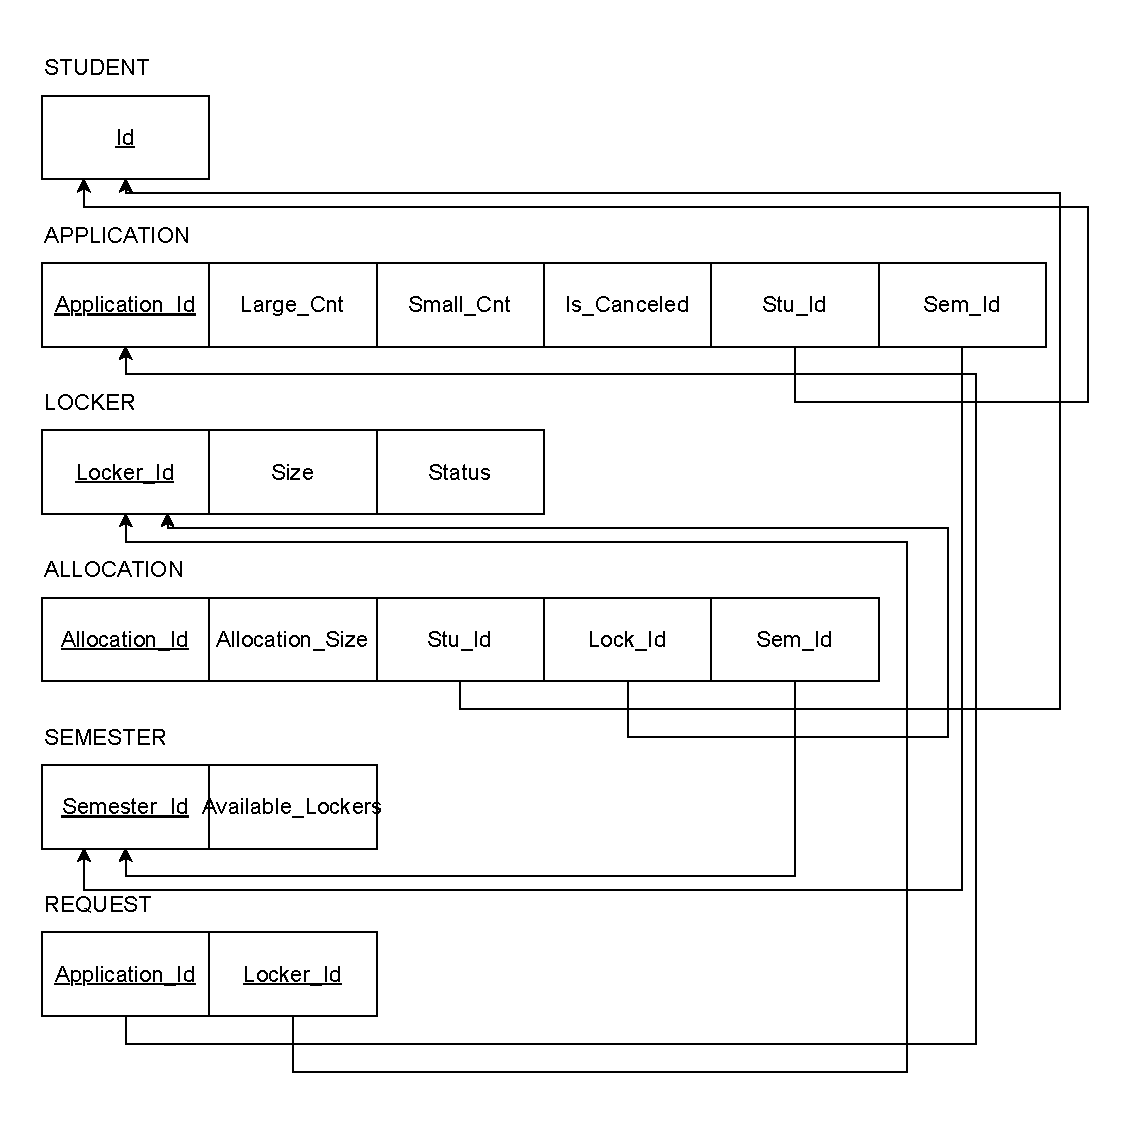
\includegraphics[width=0.8\textwidth]{2_b.png}  % 調整圖片寬度,並插入圖片檔
    \caption{Avg Time per Question v.s. Total Correct Rate}  % 可選的圖片標題
    \label{fig:2_b_image}  % 可選的標籤,用於交叉引用
\end{figure}


\subsection*{(c)}
下面有兩段程式碼分別是任務 i 和任務 ii 的程式碼。\\

下面這一段程式碼按照任務 i 的敘述依序執行。
\begin{minted}[bgcolor=lightgray, linenos, breaklines=true]{python}
import pandas as pd
import time

answers_df = pd.read_csv('./OnlineLearning_csv/answers.csv')
subscriptions_df = pd.read_csv('./OnlineLearning_csv/subscriptions.csv')

start_time = time.time()

merged_df = pd.merge(answers_df, subscriptions_df, left_on='UserID', right_on='SubscriberID')

filtered_df = merged_df[
    (merged_df['CreatedAt_x'] >= '2021-05-01') & 
    (merged_df['CreatedAt_x'] > merged_df['EndedAt'])
]

selected_columns = filtered_df[['AnswerID', 'UserID', 'QuestionID', 'MissionID', 'IsCorrect', 'CostTime', 'CreatedAt_x', 'EndedAt']]

selected_columns.rename(columns={'CreatedAt_x': 'CreatedAt'}, inplace=True)

print(selected_columns.head())

end_time = time.time()

print(f"Time taken: {end_time - start_time} seconds")
\end{minted}

而下面這一段程式碼則按照任務 ii 的敘述依序執行。
\begin{minted}[bgcolor=lightgray, linenos, breaklines=true, frame=none]{python}
import pandas as pd
import time

answers_df = pd.read_csv('./OnlineLearning_csv/answers.csv')
subscriptions_df = pd.read_csv('./OnlineLearning_csv/subscriptions.csv')

start_time = time.time()

filtered_answers_df = answers_df[answers_df['CreatedAt'] >= '2021-05-01']

merged_df = pd.merge(filtered_answers_df, subscriptions_df, left_on='UserID', right_on='SubscriberID')

final_filtered_df = merged_df[merged_df['CreatedAt_x'] > merged_df['EndedAt']]


selected_columns = final_filtered_df[['AnswerID', 'UserID', 'QuestionID', 'MissionID', 'IsCorrect', 'CostTime', 'CreatedAt_x', 'EndedAt']]

print(selected_columns.head())

end_time = time.time()

print(f"Time taken: {end_time - start_time} seconds")
\end{minted}

執行完上面兩段程式碼之後比較任務 i 和任務 ii 的執行時間,得到的結果如 Table \ref{fig:2_c_table} 所示,任務 i 的執行時間是任務 ii 的將近五倍。
\begin{table}[H]
\centering
\begin{tabular}{cc}
\toprule
Task & Time  \\
\midrule
i & 0.8418  \\
ii & 0.1497 \\
\bottomrule
\end{tabular}
\caption{}
\label{fig:2_c_table}
\end{table}
推測任務 i 的執行時間明顯長於任務 ii 的原因為任務 i 會先把整個資料表合併起來再做篩選;而任務 ii 則是先篩選再把表合併起來,透過這種方式可以合併比較少資料。由於合併資料表會花比較多時間,所以表裡面的資料數量很多的話那任務 i 的執行時間就會長很多。


\section*{3}
\subsection*{(a)}
下面是正規化完的 Schema,這個 Schema 沒有 multi-valued attributes,所有非主鍵屬性完全依賴於主鍵,不存在 transitive dependency,每個 determinant 都是 superkey,沒有 mulit-valued dependency,所以滿足 1 NF, 2 NF, 3 NF, BCNF, 及 4 NF。
% EMPLOYEE_CHECK
\begin{table}[H]
    \centering
      \textbf{Employee\_Check} \\
      \begin{tabular}{|c|c|c|c|c|}
        \hline
        \underline{employee\_id} & \underline{work\_date} & off\_type & check\_in\_time & check\_out\_time \\
        \hline
        \end{tabular}
\end{table}
  % CHECK_OUT_REASON
  \begin{table}[H]
    \centering
      \textbf{Service} \\
      \begin{tabular}{|c|c|c|c|}
        \hline
        \underline{employee\_id} & \underline{work\_date} & \underline{check\_out\_time} & reason \\
        \hline
        \end{tabular}
\end{table}

  
  % VISIT_CUSTOMER
  \begin{table}[H]
    \centering
      \textbf{Visit\_Customer} \\
      \begin{tabular}{|c|c|c|c|}
        \hline
        \underline{employee\_id} & \underline{work\_date} & \underline{check\_out\_time} & \underline{customer\_id} \\
        \hline
        \end{tabular}
      \end{table}
  



\subsection*{(b)}
原本的 relation 就是 2NF 了,因為所有的 nonprime attribute 都依賴於 prime attribute。但不是 3 NF 因為 Fee 依賴 ServiceType,而 ServiceType 又依賴 (EngineerID, CustomerID, ConsultingDate),所以把它正規化成 3 NF。\\
% 輸出 Consulting 表

\begin{table}[H]
    \centering
      \textbf{Consulting} \\
      \begin{tabular}{|c|c|c|c|}
        \hline
        \underline{EngineerID} & \underline{CustomerID} & \underline{ConsultingDate} & ServiceType \\
        \hline
        \end{tabular}
\end{table}

    



% 輸出 Service 表

\begin{table}[H]
    \centering
      \textbf{Service} \\
      \begin{tabular}{|c|c|}
        \hline
        \underline{ServiceType} & Fee \\
        \hline
        \end{tabular}
\end{table}

這樣就不會有 $X \rightarrow Z$ and $Z \rightarrow Y$ 的關係了。



\subsection*{(c)}
設計出的 Schema 如下:
% 輸出 Product 表
\begin{table}[H]
    \centering
    \textbf{Product} \\
    \begin{tabular}{|c|c|c|c|c|}
        \hline
        \underline{ProductID} & ProductName & Length & Width & Height \\
        \hline
    \end{tabular}
\end{table}

% 輸出 Supplier 表
\begin{table}[H]
    \centering
    \textbf{Supplier} \\
    \begin{tabular}{|c|c|}
        \hline
        \underline{SupplierID} & SupplierName \\
        \hline
    \end{tabular}
\end{table}

% 輸出 Pricing 表
\begin{table}[H]
    \centering
    \textbf{Pricing} \\
    \begin{tabular}{|c|c|c|c|}
        \hline
        \underline{ProductID} & \underline{SupplierID} & \underline{EffectiveDate} & Price\\
        \hline
    \end{tabular}
\end{table}

\noindent 沒有 multi-valued attributes 所以滿足 1 NF。所有非主鍵屬性完全依賴於主鍵,滿足 2 NF。不存在 transitive dependency,滿足 3 NF。每個 determinant 都是 superkey,滿足 BCNF。沒有 mulit-valued dependency,滿足 4 NF。


\section*{4}
\subsection*{(a)}
直接使用 SQL 下 query 可以有更好的效率,而且在操作上也會比較靈活,在對性能注重的地方會需要直接用 SQL。但 SQL 的程式碼比較難閱讀,而且重複性高,更有可能會受到 SQL injection 的攻擊。

使用 ORM 的好處是可以防止像是 SQL injection 的攻擊,還可以減少開發者的工作量,另外可以對不同的資料庫操作。缺點是 ORM 的查詢性能沒有 SQL 好,而且學習的成本比較高,對於複雜的查詢靈活度會受限。

\subsection*{(b)}
除了 SQL injection 之外還有一種攻擊叫資料庫暴力破解,這種攻擊方式會生成大量的用戶名和密碼組合以猜測用戶的登入資料,反覆嘗試直到成功登入。可以通過限制帳戶登入、多重驗證、監控異常流量等方式進行防範。


\subsection*{(c)}
兩者的意思是不太一樣的。「前端與後端切開」的前端意思是負責呈現資料、接收用戶輸入、處理用戶交互的部分;後端則是接收來自前端的請求、處理業務邏輯、從資料庫中檢索或存儲資料的部分。「client 端和 server 端切開」的 client 端主要是在用戶設備上執行的應用程序;server 端主要是在伺服器上執行的應用程序。所以前者主要關注 UI 與業務邏輯的分離,後者主要關注設備與服務的交互。


\end{document}
